\documentclass{article}
\usepackage[T1]{fontenc}
\usepackage{lmodern}
\usepackage{graphicx}
\usepackage{amsmath,amssymb}
\usepackage[a4paper,margin=2cm]{geometry}
\usepackage[absolute,overlay]{textpos}
\setlength{\TPHorizModule}{1mm}
\setlength{\TPVertModule}{1mm}
\usepackage[indonesian]{babel}
\usepackage{hyperref}
\setlength{\emergencystretch}{2em}
% unit: Halaman 48

\begin{document}

% === Halaman 48 (llm) ===

\vspace{238.79mm}

\begin{itemize}
    \item Kelemahan \textit{Double DES}: serangan \textit{meet-in-the-middle attack}:
    \item Dari pengamatan,
    \[ C = E_{K2}(E_{K1}(P)) \]
    maka
    \[ X = E_{K1}(P) = D_{K2}(C) \]
\end{itemize}

\vspace{40mm}

\begin{itemize}
    \item Misalkan kriptanalisis memiliki potongan $C$ dan $P$ yang berkorepsonden (\textit{known-plaintext attack}).
    \item Enkripsi $P$ untuk semua kemungkinan nilai $K1$ (yaitu sebanyak $2^{56}$ kemungkinan kunci). Hasilnya adalah semua nilai $X$
    \item Simpan semua nilai $X$ ini di dalam tabel
\end{itemize}

% deskripsi: Diagram proses enkripsi dan dekripsi Double DES yang menunjukkan serangan meet-in-the-middle, dengan aliran P ke C melalui enkripsi dua tahap (K1, K2) dan aliran C ke P melalui dekripsi dua tahap (K2, K1), bertemu di nilai perantara X.
% bbox normalisasi: [0.0600, 0.1080, 0.9400, 0.9120]
\begin{textblock*}{184.80mm}(12.60mm,32.08mm)
\noindent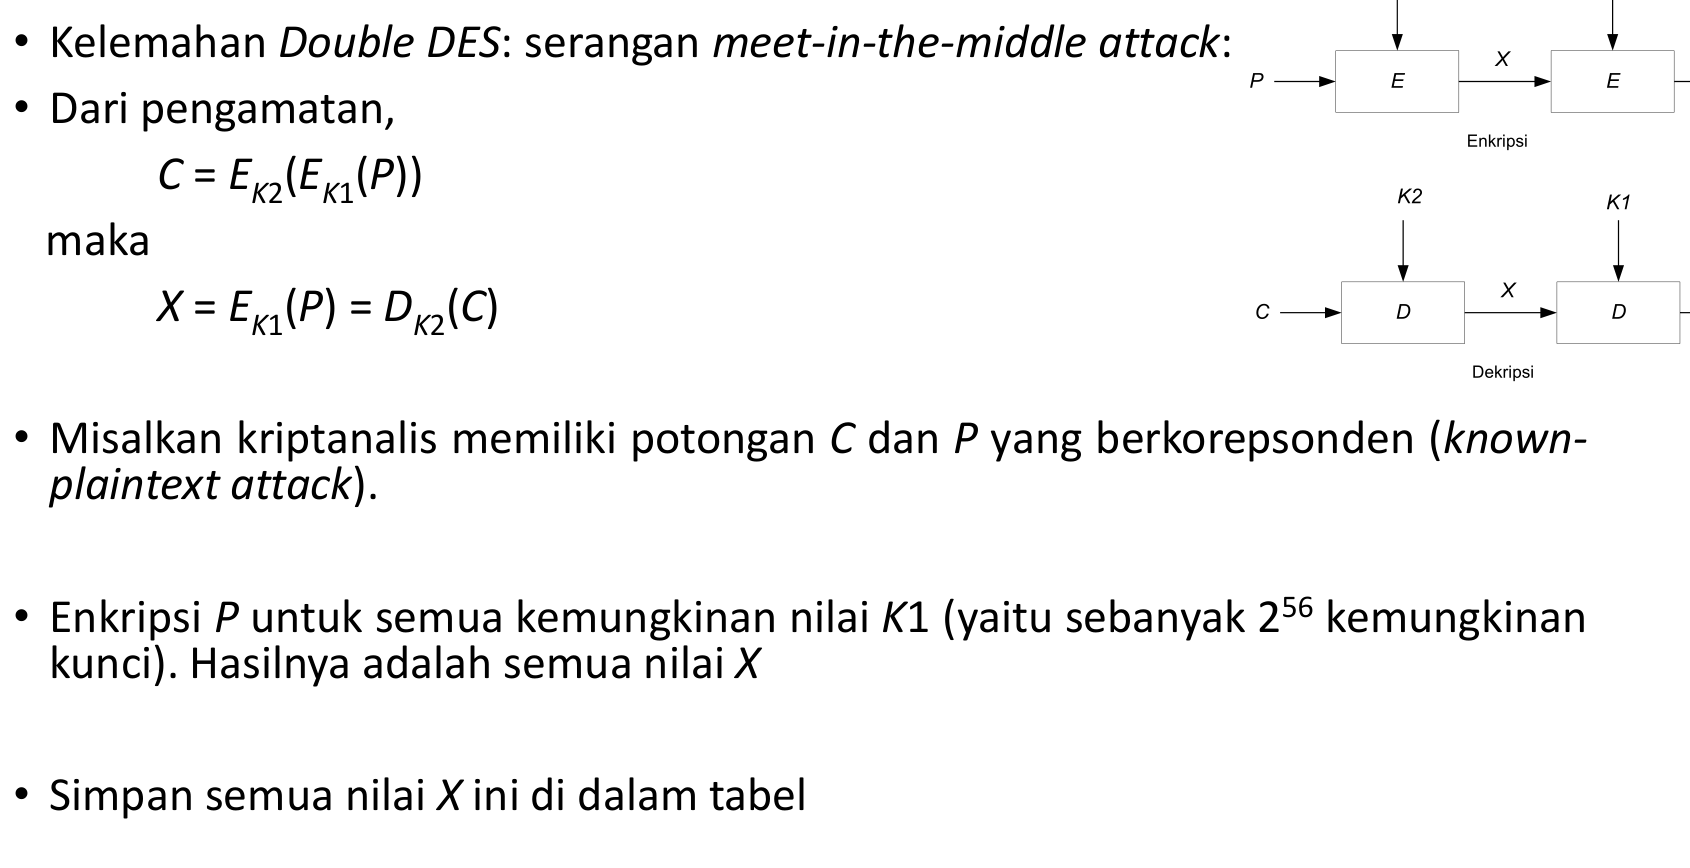
\includegraphics[width=184.80mm,height=238.79mm]{../../images/llm/page_048_img_01.png}%
\end{textblock*}

% bbox perkiraan otomatis: Diagram proses enkripsi dan dekripsi Double DES yang menunjukkan serangan meet-in-the-middle, dengan aliran P ke C melalui enkripsi dua tahap (K1, K2) dan aliran C ke P melalui dekripsi dua tahap (K2, K1), bertemu di nilai perantara X.

\end{document}
